\def\w#1{\texttt{#1}}
\def\a#1#2#3{
	\texttt{\phantom{#3}ableitbar(}#1\w{,}#2\w{)}
}
Die Grammatik
\begin{align*}
S_0& \to NE \mid NA \mid \varepsilon \\
S  & \to NE \mid NA \\
A  &\to SE \\
N&\to \w{0} \\
E&\to \w{1} 
\end{align*}
für Wörter der Form
$\w{0}^n\w{1}^n$
hat Chomsky-Normalform.
\begin{teilaufgaben}
\item
Verfolgen Sie mit Hilfe des Pseudocode, welche Aufrufe der Funktion
\w{ableitbar} der CYK-Algorithmus durchführen wird, wenn 
$\a{S_0}{\w{0011}}{}$ aufgerufen wird.
\item 
Leiten Sie daraus den Parse Tree ab.
\end{teilaufgaben}


\begin{loesung}
Der CYK-Algorithmus verwendet rekursive Aufrufe der Funktion
\texttt{ableitbar}, um herauszufinden, ob ein Teilwort aus einer 
Variablen ableitbar ist.
Die Gesamtheit der Aufrufe ist in Tabelle~\ref{40000082:loesung}
zusammengestellt.
Um die spätere Diskussion zu vereinfachen, überlegen wir uns zunächst
ein paar Spezialfälle.

Das leere Wort ist nur aus der Startvariablen ableitbar, daher ist
$\a{A}{\varepsilon}{}$ nur dann wahr, wenn $A=S_0$ ist.

Hat das Wort $w$ die Länge $1$, dann ist 
$\a{A}{w}{}$ nur wahr
für $A=N$ und $w=\texttt{0}$
bzw.~für $A=E$ und $w=\texttt{1}$.

Der erste Aufruf der Funktion \texttt{ableitbar} fragt, ob das Wort
\texttt{0011} aus $S_0$ ableitbar ist.
Dazu muss zunächst kontrolliert werden, ob das leere Wort vorliegt,
dies ist hier nicht der Fall.
Dann kommen die Zweierregeln dran, die Regeln
$S_0\to NE$
und
$S_0\to NA$.
Für beide müssen die Unterteilungen
\texttt{0|011},
\texttt{00|11} oder
\texttt{001|1}
daraufhin getestet werden, ob die Teile aus $N$ bzw.~$E$ oder $A$
ableitbar sind:
\begin{itemize}
\item
\texttt{0|011}:
Es muss $\a{N}{\texttt{0}}{}$ und $\a{E}{\texttt{011}}{}$ 
aufgerufen werden.
Der erste Aufruf ist erfolgreich, aber der zweite gibt {\em false} zurück,
so dass diese Unterteilung nicht in Frage kommt.
\item
\texttt{00|11}: muss nicht mehr aufgerufen werden.
Es muss $\a{N}{\texttt{00}}{}$ und $\a{E}{\texttt{11}}{}$
aufgerufen werden.
Bereits der erste Aufruf gibt {\em false} zurück.
\item
\texttt{001|1}: muss nicht mehr aufgerufen werden.
Es muss $\a{N}{\texttt{001}}{}$ und $\a{E}{\texttt{1}}{}$
aufgerufen werden.
Bereits der erste Aufruf gibt {\em false} zurück, da nützt es auch
nichts, dass der zweite {\em true} ergeben würde..
\end{itemize}
Damit ist die Regel $S_0\to NE$ ausgeschlossen und es kann $S_0\to NA$
versucht werden.
\begin{itemize}
\item
\texttt{0|011}:
Es muss $\a{N}{\texttt{0}}{}$ und $\a{A}{\texttt{011}}{}$ 
aufgerufen werden.
Der erste Aufruf ist wieder erfolgreich, es kommt jetzt also auf den
zweiten an.
Darin werden die Unterteilungen \texttt{0|11} und \texttt{01|1}
mit der Regel $A\to SE$ probiert.
\begin{itemize}
\item
\texttt{0|11}: Der Aufruf $\a{E}{\texttt{11}}{}$ gibt {\em false}
zurück.
\item
\texttt{01|1}: Der Aufruf $\a{E}{\texttt{1}}{}$ gibt {\em true}
zurück, es ist also nur noch der Rückgabewert von $\a{S}{\texttt{01}}{}$
zu prüfen.
Dabei wird die Regel $S\to NE$ verwendet, die auf die Aufrufe
\a{N}{\texttt{0}}{}
und
\a{E}{\texttt{1}}{}
führt, die beide {\em true} zurückgeben.
Damit ist gefunden, dass das Wort ableitbar ist.
\end{itemize}
\end{itemize}
Aus der Liste der erfolgreichen Aufrufe kann man auch den Parse Tree
ablesen.
Die erste Regel ist $S_0\to NA$, als nächste Regel wird $A\to SE$ angewendet
und schliesslich $S\to NE$.
Dies ergibt den Parse Tree
\begin{center}
\def\pfeil#1#2{\draw[->,shorten >= 0.25cm,shorten <= 0.25cm] #1 -- #2;}
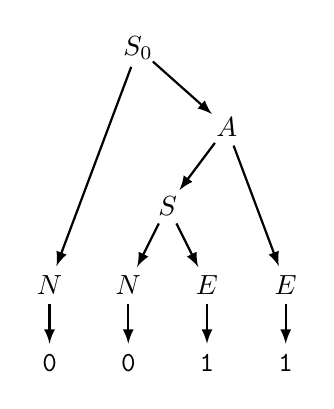
\begin{tikzpicture}[>=latex,thick]
\def\l{1}
\coordinate (T0) at ({-1.5*\l},0);
\coordinate (T1) at ({-0.5*\l},0);
\coordinate (T2) at ({0.5*\l},0);
\coordinate (T3) at ({1.5*\l},0);
\coordinate (S0) at ({-1.5*\l},{\l});
\coordinate (S1) at ({-0.5*\l},{\l});
\coordinate (S2) at ({0.5*\l},{\l});
\coordinate (S3) at ({1.5*\l},{\l});
\coordinate (S4) at (0,{2*\l});
\coordinate (A0) at ({0.75*\l},{3*\l});
\coordinate (S5) at ({-0.375*\l},{4*\l});
\node at (T0) {\texttt{0}};
\node at (T1) {\texttt{0}};
\node at (T2) {\texttt{1}};
\node at (T3) {\texttt{1}};
\node at (S0) {$N$};
\node at (S1) {$N$};
\node at (S2) {$E$};
\node at (S3) {$E$};
\node at (S4) {$S$};
\node at (A0) {$A$};
\node at (S5) {$S_0$};
\pfeil{(S0)}{(T0)}
\pfeil{(S1)}{(T1)}
\pfeil{(S2)}{(T2)}
\pfeil{(S3)}{(T3)}
\pfeil{(S4)}{(S1)}
\pfeil{(S4)}{(S2)}
\pfeil{(A0)}{(S4)}
\pfeil{(A0)}{(S3)}
\pfeil{(S5)}{(S0)}
\pfeil{(S5)}{(A0)}
\end{tikzpicture}
\end{center}
\begin{table}
\centering
\def\c#1{\multicolumn{1}{|c}{#1}}
\def\C#1{\multicolumn{1}{|c|}{#1}}
\begin{tabular}{>{$}l<{$}>{$}l<{$}>{$}l<{$}>{$}l<{$}|>{$}r<{$}>{$}l<{$}|>{$}l<{$}|>{$}l<{$}|>{$}c<{$}|}
\hline
\multicolumn{4}{|c|}{\text{Ebene}}&\multicolumn{2}{c|}{Unterteilung}&\text{Regel}&\text{Aufruf}&\text{Resultat}\\
\hline
\c{0}&&&&        &        &         &\a{S_0}{\w{0011}}{}  &\checkmark \\
\cline{1-1}
\cline{5-9}
&\c{1}&&&   \w{0}&\w{011} &S_0\to NE&\a{N}{\w{0}}{00}     &\checkmark \\
&\c{ }&&&        &        &         &\a{E}{\w{011}}{00}   &\times     \\
\cline{7-9}
&\c{ }&&&        &        &S_0\to NA&\a{N}{\w{0}}{00}     &\checkmark \\
&\c{ }&&&        &        &         &\a{A}{\w{011}}{00}   &\times     \\
\cline{2-2}
\cline{5-9}
&&\c{2}&&   \w{0}&\w{11}  &A\to SE  &\a{S}{\w{0}}{0000}   &\times     \\
&&\c{ }&&        &        &         &\a{E}{\w{11}}{0000}  &\times     \\
\cline{5-9}
&&\c{ }&&  \w{01}&\w{1}   &A\to SE  &\a{S}{\w{01}}{0000}  &\checkmark \\
\cline{3-3}
\cline{5-9}
&&&\C{3}&   \w{0}&\w{1}   &S\to NE  &\a{N}{\w{0}}{000000} &\checkmark \\
&&&\C{ }&        &        &         &\a{E}{\w{1}}{000000} &\checkmark \\
\cline{3-3}
\cline{5-9}
&&\c{2}&&  \w{01}&\w{1}   &A\to SE  &\a{E}{\w{1}}{0000}   &\checkmark \\
\cline{3-3}
\cline{5-9}
&&&\C{3}&   \w{0}&\w{1}   &S\to NE  &\a{N}{\w{0}}{000000} &\checkmark \\
\cline{4-9}
\end{tabular}
\caption{Aufrufe der Funktion $\a{V}{w}{}$ nach dem CYK-Algorithmus,
die der Aufruf von $\a{S_0}{\w{0011}}{}$ zur Folge hat (Lösung von
Aufgabe~\ref{40000082}
\label{40000082:loesung}}
\end{table}
\end{loesung}
